\documentclass[10pt]{article}
\usepackage[margin=1in]{geometry}
\usepackage[T1]{fontenc}
\usepackage{lmodern,microtype,amsmath,amssymb,booktabs,graphicx,xcolor}
\usepackage[numbers,sort&compress]{natbib}
\usepackage[colorlinks=true,linkcolor=blue!50!black,citecolor=blue!50!black,urlcolor=blue!50!black]{hyperref}
% AUTO-GENERATED by scripts/make_numbers.py from results/ -- do not edit
\newcommand{\AntiFID}{143.3 $\pm$ 3.0}
\newcommand{\AntiFIDdiff}{+2.3}
\newcommand{\AntiFIDpair}{2.3 $\pm$ 4.3}
\newcommand{\AntiHO}{37.75 $\pm$ 0.02}
\newcommand{\AntiHOdiff}{+0.7}
\newcommand{\AntiHOpair}{0.7 $\pm$ 0.4}
\newcommand{\AntiMS}{91.0}
\newcommand{\AntiOvh}{+0.2}
\newcommand{\AntiSeeds}{3}
\newcommand{\AntiVR}{0.92 $\pm$ 0.08}
\newcommand{\AntiVRall}{1.16}
\newcommand{\AntiVRbelow}{2/8}
\newcommand{\AntiVRmax}{1.46}
\newcommand{\AntiVRmin}{0.84}
\newcommand{\AntipFID}{0.58}
\newcommand{\AntipFIDpair}{0.45}
\newcommand{\AntipHO}{0.14}
\newcommand{\AntipHOpair}{0.12}
\newcommand{\DecE}{50}
\newcommand{\DecLHS}{0.50}
\newcommand{\DecN}{3}
\newcommand{\DecRHS}{0.36}
\newcommand{\DecStep}{3000}
\newcommand{\DecT}{6}
\newcommand{\DecX}{44}
\newcommand{\Decoracle}{0.62}
\newcommand{\DecpAnti}{1.15}
\newcommand{\DecpPaired}{1.50}
\newcommand{\DecpSA}{1.03}
\newcommand{\DecpStrat}{0.94}
\newcommand{\Decrho}{-0.71}
\newcommand{\FAntiHO}{57.89 $\pm$ 0.87}
\newcommand{\FAntiHOdiff}{+1.7}
\newcommand{\FAntiHOpair}{1.7 $\pm$ 0.9}
\newcommand{\FAntiMS}{3123.1}
\newcommand{\FAntiOvh}{+0.4}
\newcommand{\FAntiSeeds}{3}
\newcommand{\FAntiVR}{1.40 $\pm$ 0.12}
\newcommand{\FAntiVRall}{1.41}
\newcommand{\FAntiVRbelow}{0/6}
\newcommand{\FAntiVRmax}{1.67}
\newcommand{\FAntiVRmin}{1.25}
\newcommand{\FAntipHO}{0.21}
\newcommand{\FAntipHOpair}{0.09}
\newcommand{\FDecE}{31}
\newcommand{\FDecLHS}{0.69}
\newcommand{\FDecN}{3}
\newcommand{\FDecRHS}{0.24}
\newcommand{\FDecStep}{800}
\newcommand{\FDecT}{6}
\newcommand{\FDecX}{63}
\newcommand{\FDecoracle}{0.47}
\newcommand{\FDecpAnti}{1.45}
\newcommand{\FDecpPaired}{1.69}
\newcommand{\FDecpSA}{1.33}
\newcommand{\FDecpStrat}{0.94}
\newcommand{\FDecrho}{-0.78}
\newcommand{\FGradRange}{18}
\newcommand{\FISSVR}{0.64 $\pm$ 0.07}
\newcommand{\FISSVRall}{0.60}
\newcommand{\FISSVRbelow}{6/6}
\newcommand{\FISSVRmax}{0.71}
\newcommand{\FISSVRmin}{0.49}
\newcommand{\FImpHO}{54.98}
\newcommand{\FImpHOdiff}{-3.4}
\newcommand{\FImpMS}{3190.1}
\newcommand{\FImpOvh}{+2.5}
\newcommand{\FImpSeeds}{1}
\newcommand{\FImpVR}{0.58 $\pm$ 0.03}
\newcommand{\FImpVRall}{0.62}
\newcommand{\FImpVRbelow}{6/6}
\newcommand{\FImpVRmax}{0.81}
\newcommand{\FImpVRmin}{0.55}
\newcommand{\FImppHO}{n/a}
\newcommand{\FLossRange}{136}
\newcommand{\FPairedVR}{2.31 $\pm$ 0.10}
\newcommand{\FPairedVRall}{1.81}
\newcommand{\FPairedVRbelow}{0/6}
\newcommand{\FPairedVRmax}{2.41}
\newcommand{\FPairedVRmin}{1.32}
\newcommand{\FProbeN}{6}
\newcommand{\FProbeSteps}{200, 800}
\newcommand{\FSAHO}{56.55}
\newcommand{\FSAHOdiff}{-0.7}
\newcommand{\FSAMS}{3070.7}
\newcommand{\FSAOvh}{-1.3}
\newcommand{\FSASeeds}{1}
\newcommand{\FSAVR}{1.16 $\pm$ 0.03}
\newcommand{\FSAVRall}{0.95}
\newcommand{\FSAVRbelow}{3/6}
\newcommand{\FSAVRmax}{1.19}
\newcommand{\FSAVRmin}{0.71}
\newcommand{\FSApHO}{n/a}
\newcommand{\FSobolVR}{0.80 $\pm$ 0.08}
\newcommand{\FSobolVRall}{0.78}
\newcommand{\FSobolVRbelow}{6/6}
\newcommand{\FSobolVRmax}{0.89}
\newcommand{\FSobolVRmin}{0.73}
\newcommand{\FSteps}{800}
\newcommand{\FStratHO}{56.23 $\pm$ 0.29}
\newcommand{\FStratHOdiff}{-1.2}
\newcommand{\FStratHOpair}{-0.6 $\pm$ 0.0}
\newcommand{\FStratMS}{3144.3}
\newcommand{\FStratOvh}{+1.0}
\newcommand{\FStratSeeds}{2}
\newcommand{\FStratVR}{0.95 $\pm$ 0.03}
\newcommand{\FStratVRall}{0.85}
\newcommand{\FStratVRbelow}{6/6}
\newcommand{\FStratVRmax}{0.98}
\newcommand{\FStratVRmin}{0.72}
\newcommand{\FStratpHO}{0.21}
\newcommand{\FStratpHOpair}{0.03}
\newcommand{\FUnbiasMax}{2.50}
\newcommand{\FUnbiasMean}{0.84}
\newcommand{\FUnbiasMin}{0.34}
\newcommand{\FUnbiasN}{42}
\newcommand{\FUnifHO}{56.93 $\pm$ 0.66}
\newcommand{\FUnifHOdiff}{+0.0}
\newcommand{\FUnifMS}{3111.9}
\newcommand{\FUnifOvh}{+0.0}
\newcommand{\FUnifSeeds}{3}
\newcommand{\FUnifpHO}{1.00}
\newcommand{\GPUhours}{1.97}
\newcommand{\GPUhoursLost}{0.42}
\newcommand{\GradRange}{8}
\newcommand{\ISSVR}{0.89 $\pm$ 0.02}
\newcommand{\ISSVRall}{0.78}
\newcommand{\ISSVRbelow}{7/8}
\newcommand{\ISSVRmax}{1.04}
\newcommand{\ISSVRmin}{0.52}
\newcommand{\ImpFID}{135.3 $\pm$ 4.1}
\newcommand{\ImpFIDdiff}{-5.7}
\newcommand{\ImpFIDpair}{-5.7 $\pm$ 2.7}
\newcommand{\ImpHO}{36.92 $\pm$ 0.32}
\newcommand{\ImpHOdiff}{-1.5}
\newcommand{\ImpHOpair}{-1.5 $\pm$ 0.8}
\newcommand{\ImpMS}{92.2}
\newcommand{\ImpOvh}{+1.5}
\newcommand{\ImpSeeds}{3}
\newcommand{\ImpVR}{1.22 $\pm$ 0.34}
\newcommand{\ImpVRall}{0.84}
\newcommand{\ImpVRbelow}{5/8}
\newcommand{\ImpVRmax}{1.61}
\newcommand{\ImpVRmin}{0.51}
\newcommand{\ImppFID}{0.24}
\newcommand{\ImppFIDpair}{0.06}
\newcommand{\ImppHO}{0.07}
\newcommand{\ImppHOpair}{0.08}
\newcommand{\LossRange}{190}
\newcommand{\MDEd}{3.1}
\newcommand{\MDEfid}{12}
\newcommand{\MDEho}{1.7}
\newcommand{\PairedVR}{1.22 $\pm$ 0.08}
\newcommand{\PairedVRall}{1.47}
\newcommand{\PairedVRbelow}{0/8}
\newcommand{\PairedVRmax}{1.76}
\newcommand{\PairedVRmin}{1.13}
\newcommand{\ProbeN}{8}
\newcommand{\ProbeSteps}{250, 1000, 2000, 3000}
\newcommand{\SAFID}{141.2 $\pm$ 3.7}
\newcommand{\SAFIDdiff}{+0.2}
\newcommand{\SAFIDpair}{-3.0 $\pm$ 4.1}
\newcommand{\SAHO}{37.65 $\pm$ 0.19}
\newcommand{\SAHOdiff}{+0.4}
\newcommand{\SAHOpair}{0.4 $\pm$ 0.7}
\newcommand{\SAMS}{89.4}
\newcommand{\SAOvh}{-1.6}
\newcommand{\SASeeds}{3}
\newcommand{\SAVR}{0.83 $\pm$ 0.04}
\newcommand{\SAVRall}{0.96}
\newcommand{\SAVRbelow}{5/8}
\newcommand{\SAVRmax}{1.11}
\newcommand{\SAVRmin}{0.80}
\newcommand{\SApFID}{0.96}
\newcommand{\SApFIDpair}{0.49}
\newcommand{\SApHO}{0.37}
\newcommand{\SApHOpair}{0.43}
\newcommand{\SobolVR}{0.86 $\pm$ 0.01}
\newcommand{\SobolVRall}{0.83}
\newcommand{\SobolVRbelow}{8/8}
\newcommand{\SobolVRmax}{0.87}
\newcommand{\SobolVRmin}{0.77}
\newcommand{\Steps}{3000}
\newcommand{\StratFID}{140.0 $\pm$ 2.8}
\newcommand{\StratFIDdiff}{-1.0}
\newcommand{\StratFIDpair}{-1.0 $\pm$ 3.0}
\newcommand{\StratHO}{37.70 $\pm$ 0.22}
\newcommand{\StratHOdiff}{+0.5}
\newcommand{\StratHOpair}{0.5 $\pm$ 0.7}
\newcommand{\StratMS}{90.4}
\newcommand{\StratOvh}{-0.5}
\newcommand{\StratSeeds}{3}
\newcommand{\StratVR}{0.82 $\pm$ 0.03}
\newcommand{\StratVRall}{0.82}
\newcommand{\StratVRbelow}{8/8}
\newcommand{\StratVRmax}{0.89}
\newcommand{\StratVRmin}{0.76}
\newcommand{\StratpFID}{0.80}
\newcommand{\StratpFIDpair}{0.61}
\newcommand{\StratpHO}{0.29}
\newcommand{\StratpHOpair}{0.29}
\newcommand{\UnbiasMax}{2.50}
\newcommand{\UnbiasMean}{0.83}
\newcommand{\UnbiasMin}{0.34}
\newcommand{\UnbiasN}{98}
\newcommand{\UnifFID}{141.0 $\pm$ 5.7}
\newcommand{\UnifFIDdiff}{+0.0}
\newcommand{\UnifHO}{37.50 $\pm$ 0.18}
\newcommand{\UnifHOdiff}{+0.0}
\newcommand{\UnifMS}{90.8}
\newcommand{\UnifOvh}{+0.0}
\newcommand{\UnifSeeds}{3}
\newcommand{\UnifpFID}{1.00}
\newcommand{\UnifpHO}{1.00}

\newcommand{\ttt}[1]{\texttt{#1}}
\title{Monte Carlo Variance Reduction for Diffusion-Model Training:\\
an Equal-Compute Comparison of Antithetic, Stratified and Importance Sampling}
\author{Research project report (single author)\\\small Code, logs and every number: \url{https://github.com/polylam1994/Monte-Carlo-variance-reduction-for-diffusion-model-training}}
\date{November 2026}
\begin{document}
\maketitle

\begin{abstract}
The DDPM training loss is a Monte Carlo average over data, timesteps and Gaussian noise, so standard
variance-reduction methods from computational finance apply directly. We test whether they help, at equal
compute, in a single controlled codebase. The arms are antithetic noise pairs $(\epsilon,-\epsilon)$, stratified and
scrambled-Sobol timesteps, Improved-DDPM-style importance sampling of timesteps, and stratified timesteps with
antithetic noise. Only the $(x_0,t,\epsilon)$ estimator changes, and every step uses 128 evaluations. We
measure gradient variance directly at fixed parameters and decompose it by the law of total variance into
between-timestep, data and noise parts. On CIFAR-10 the between-timestep part is only \DecT\% of the total, so
stratification removes little variance (variance ratio \StratVR\ at the final checkpoint, with no measurable
overhead). Antithetic pairs are strongly anti-correlated (pooled $\rho=\Decrho$), but each pair shares one
image and one timestep, and that cost outweighs the cancellation (ratio \AntiVR). The loss-based importance
proposal over-weights low-noise timesteps. On CIFAR-10 it reduces variance early in training but increases it
later (ratio \ImpVRmin--\ImpVRmax\ across checkpoints); a gradient-norm oracle proposal is predicted to give \Decoracle.
None of these variance changes produced a statistically significant improvement in held-out loss or FID after
\Steps\ steps with 3 seeds. The decomposition predicts the sign of each effect before any training, which is
the main practical result.
\end{abstract}

\section{Introduction}
Pricing an option by simulation and training a diffusion model have the same structure. In both, an expectation
over random inputs is replaced by a sample average, and the error of that average limits progress. In finance,
decades of work have produced methods that cut that error at almost no extra cost
\citep{glasserman2003,boyle1977,paskov1995,ghs1999}. Denoising score matching \citep{ho2020ddpm} is the same
kind of average, over data, timesteps $t$ and noise $\epsilon$, and the gradient noise it injects into SGD is
thought to slow training \citep{kim2025adaptive}. This report asks one concrete question: \emph{does
plugging these classical estimators into DDPM training reduce gradient variance, and does that make training
faster or better at equal compute?}

\paragraph{What is and is not new.} Importance sampling of timesteps is established
\citep{nichol2021improved,song2021mle,kim2025adaptive,sun2026variance}, and stratified or low-discrepancy
timesteps are used in VDM \citep{kingma2021vdm} and CARV \citep{carv2026}. For these arms we replicate under
controlled conditions. We did not find antithetic $\epsilon$-pairs inside the DDPM training estimator in
prior work: antithetic noise has been used at sampling time \citep{antithetic2026}, and antithetic couplings for
other gradient estimators \citep{ren2019antithetic}. The closest work on control variates for the DDPM gradient
\citep{jeha2024taylor} found inconclusive effects on MNIST. Our contributions are:
(1) an equal-compute comparison in one codebase where only the estimator changes, on Fashion-MNIST and CIFAR-10
with three seeds;
(2) direct measurement of gradient variance at identical parameters for eight estimators, with a law-of-total-variance
decomposition (Eq.~\ref{eq:decomp}) that \emph{predicts} each estimator's variance;
(3) a simple condition, $V_t+V_x<-\rho V_\epsilon$, for when antithetic noise can help, together with the
measurement that it fails here;
(4) evidence that the loss-based importance proposal is mismatched to the gradient: the loss varies by
$\approx$\LossRange$\times$ across timesteps, but gradient second moments by only $\approx$\GradRange$\times$.
All numbers in this report are generated from logged runs by scripts in the repository.

\section{Background}
\label{sec:background}

\paragraph{The DDPM objective as a Monte Carlo integral.}
With a fixed noise schedule $\bar\alpha_t$, $t\in\{0,\dots,T-1\}$, the $\epsilon$-prediction loss of
\citet{ho2020ddpm} is
\begin{equation}
  \mathcal L(\theta)=\mathbb E_{x_0\sim p_{\text{data}},\,t\sim\mathcal U\{0..T-1\},\,\epsilon\sim\mathcal N(0,I)}
  \big[\ell(\theta;x_0,t,\epsilon)\big],\qquad
  \ell=\tfrac1d\big\|\hat\epsilon_\theta(\sqrt{\bar\alpha_t}x_0+\sqrt{1-\bar\alpha_t}\,\epsilon,\,t)-\epsilon\big\|^2 .
  \label{eq:loss}
\end{equation}
Each optimiser step replaces $\nabla\mathcal L$ by an $N$-sample estimator
$\hat g=\frac1N\sum_{i=1}^N w_i\,\nabla_\theta\ell(\theta;x_0^{(i)},t^{(i)},\epsilon^{(i)})$.
The baseline draws all three inputs i.i.d.\ and sets $w_i=1$. Pricing a derivative by simulation has the
same form: an expectation of a payoff over random paths, estimated from a finite sample. Computational
finance has a standard set of tools for this \citep{glasserman2003}: antithetic variates \citep{boyle1977},
stratification and quasi-Monte Carlo \citep{paskov1995}, importance sampling \citep{ghs1999} and control
variates \citep{kemna1990}. All of them can be applied to $\hat g$ without changing
$\mathbb E\hat g=\nabla\mathcal L$.

\paragraph{Where the variance comes from.}
Write $g=\nabla_\theta\ell(\theta;x_0,t,\epsilon)$ for a per-sample gradient and measure variance by the trace of
the covariance, $\mathrm{V}(\cdot)=\mathbb E\|\cdot-\mathbb E\cdot\|^2$. The law of total variance splits it into three
non-negative parts:
\begin{equation}
  \mathrm V(g)=\underbrace{\mathrm V_t\big(\mathbb E[g\mid t]\big)}_{V_t:\ \text{between timesteps}}
  +\underbrace{\mathbb E_t\,\mathrm V_{x_0}\big(\mathbb E[g\mid x_0,t]\big)}_{V_x:\ \text{data, given }t}
  +\underbrace{\mathbb E_{x_0,t}\,\mathrm V_\epsilon\big(g\mid x_0,t\big)}_{V_\epsilon:\ \text{noise}} .
  \label{eq:decomp}
\end{equation}
Each technique below acts on a different term. This is the main analytical tool of the paper:
by measuring $V_t$, $V_x$ and $V_\epsilon$ we can predict which technique can help before training.

\section{Estimators}
\label{sec:method}
All estimators use exactly $N=128$ evaluations of $\ell$ per step (an antithetic pair counts as two), are unbiased for
$\nabla\mathcal L$, and differ only in how $(x_0,t,\epsilon,w)$ are drawn.

\paragraph{Stratified and quasi-Monte Carlo timesteps.}
\texttt{stratified} draws $u_i=(i+U_i)/N$, $U_i\sim\mathcal U[0,1)$, one point per stratum, and sets
$t_i=\lfloor Tu_i\rfloor$. Its variance is at most that of the baseline, because it removes the between-strata
part of $V_t$: $\mathrm V(\hat g_{\text{strat}})\approx (V_x+V_\epsilon+V_t^{\text{within}})/N$.
\texttt{sobol} uses consecutive points of a scrambled one-dimensional Sobol sequence. For $N=2^k$ each block of
$N$ points is a $(0,k,1)$-net, so in one dimension it is essentially a stratified sample with a
correlated scramble \citep{owen1997scrambled}, and we expect \texttt{sobol}$\approx$\texttt{stratified}.
The ``low-discrepancy sampler'' of VDM \citep{kingma2021vdm} is a randomly shifted lattice from the same
family.

\paragraph{Antithetic noise.}
\texttt{antithetic} draws $N/2$ triples $(x_0,t,\epsilon)$ and evaluates both $\epsilon$ and $-\epsilon$. With
$\rho=\mathrm{Cov}(g(\epsilon),g(-\epsilon))/V_\epsilon$ (the trace correlation of the pair, given $x_0,t$),
\begin{equation}
  \mathrm V(\hat g_{\text{anti}})=\frac{2(V_t+V_x)+(1+\rho)V_\epsilon}{N}
  \quad\text{vs.}\quad
  \mathrm V(\hat g_{\text{unif}})=\frac{V_t+V_x+V_\epsilon}{N},
  \label{eq:anti}
\end{equation}
so antithetic sampling helps if and only if $V_t+V_x<-\rho\,V_\epsilon$. In option pricing the pair shares
nothing but the normal draw, and the condition reduces to the textbook $\rho<0$. Here the pair also
shares $(x_0,t)$, so it pays for the cancellation with half as many distinct images and timesteps. If
$\hat\epsilon_\theta$ were affine in $x_t$, $g$ would be affine in $\epsilon$ and $\rho=-1$: the odd part cancels
exactly. The diagnostic estimator \texttt{paired\_iid} uses the same pairing with two independent
$\epsilon$, so the gap between \texttt{paired\_iid} and \texttt{antithetic} isolates the effect of $\rho$.
\texttt{strat\_anti} combines both ideas: the $N/2$ pair timesteps are stratified.

\paragraph{Importance-sampled timesteps.}
\texttt{importance} samples $t$ from a piecewise-constant proposal $q$ over 50 bins and reweights by
$w=1/(Tq(t))$, which leaves $\mathcal L$ unchanged \citep{kingma2023understanding}. Following Improved DDPM
\citep{nichol2021improved}, $q(t)\propto\sqrt{\mathbb E[\ell^2\mid t]}$, estimated from a 100-sample history per
bin, used after every bin is filled, and mixed 90/10 with the uniform distribution so that $w\le 10$.
This proposal minimises the variance of the \emph{loss} estimate. The proposal that minimises the
trace of the \emph{gradient} covariance is instead $q^\star(t)\propto\sqrt{\mathbb E[\|g\|^2\mid t]}$
(the same Cauchy--Schwarz argument, applied to $\|g\|$), and it can differ substantially. We report the
predicted variance under $q^\star$ as an oracle and do not train with it. \texttt{is\_strat}
pushes stratified uniforms through the inverse CDF of $q$ (as in CARV \citep{carv2026}); it is probed but
not trained.

\section{Experimental setup}
\label{sec:setup}
\paragraph{Model and training.} DDPM with $T=1000$, linear $\beta_t\in[10^{-4},0.02]$, $\epsilon$-prediction and the
unweighted loss \eqref{eq:loss}. U-Net with residual blocks, GroupNorm, SiLU, sinusoidal time embedding and one
self-attention layer at the lowest resolution. CIFAR-10 \citep{krizhevsky2009}: base width 32, multipliers
$(1,2,2)$, two blocks per level, 1.54M parameters, random horizontal flips. Fashion-MNIST \citep{xiao2017fmnist}:
width 32, multipliers $(1,2)$, one block per level, 0.63M parameters. Adam \citep{kingma2015adam}, learning
rate $2\cdot10^{-4}$ with 200 warm-up steps, gradient clipping at 1, batch $N=128$, EMA 0.999 (with the standard
warm-up on CIFAR-10), fp16 autocast on GPU. Everything except the estimator is identical across arms. For a
given seed, every estimator starts from the same initialisation.

\paragraph{Budget and equal compute.} We compare at an equal number of optimiser steps, which here also means an
equal number of network evaluations: every step uses 128 forward/backward passes through the U-Net. CIFAR-10:
3,000 steps per run (384k evaluations, $\approx$7.7 epochs) on one NVIDIA T4. Fashion-MNIST: 800 steps per run on
a 4-core CPU. Three seeds (0, 1, 2) per configuration, fixed in advance; no run was dropped. The whole study
used \GPUhours\ Kaggle GPU-hours of a 2-hour budget, including \GPUhoursLost\ GPU-hours lost to a failed data
download (Appendix~\ref{app:budget}). This budget, not the method, is the main limitation of the study
(\S\ref{sec:limitations}).

\paragraph{Metrics.}
(i) \emph{Gradient variance at fixed parameters.} Inside each baseline run, at fixed checkpoints, we freeze
$\theta$ and draw $R=48$ independent mini-batch gradients from each of the eight estimators. $x_0$ is drawn from a
fixed pool of 4,096 training images. We report $\mathrm{tr}\,\mathrm{Cov}(\hat g)$ relative to \texttt{uniform}
at the same $\theta$. All estimators share the same checkpoints, so the ratio isolates the estimator. We also check
unbiasedness: if two estimators have the same mean, $\mathbb E\|\bar g_e-\bar g_u\|^2=(\mathrm{tr}_e+\mathrm{tr}_u)/R$;
across all \UnbiasN\ estimator--checkpoint pairs the observed ratio of the two sides has mean \UnbiasMean\
(range \UnbiasMin--\UnbiasMax), so there is no sign of bias.
(ii) \emph{Decomposition} \eqref{eq:decomp} in 20 timestep bins from paired mini-batches that share or
resample $(x_0,t)$ and $\epsilon$, or flip the sign of $\epsilon$ (3 repetitions, $n=64$ per batch). It gives
$V_t$, $V_x$, $V_\epsilon$ and the pooled $\rho$, which we plug into \eqref{eq:anti} to \emph{predict} each estimator's
variance and compare with (i).
(iii) \emph{Held-out loss} on 2,000 test images with common random numbers: the same $(x_0,t,\epsilon)$ for every
model and checkpoint, the standard variance-reduction device for comparing simulated alternatives
\citep{glasserman2003}.
(iv) \emph{FID} \citep{heusel2017fid} with clean-fid \citep{parmar2022cleanfid}: 10k samples, deterministic DDIM
\citep{song2021ddim} with 25 steps from the EMA weights, and the same initial noise for every model, against
CIFAR-10 training statistics. FID is computed at steps 1k/2k/3k for seed 0 and at 3k for seeds 1--2, for budget
reasons. Absolute values are high because the models are small and briefly trained; only differences are
interpreted.
(v) \emph{Overhead}: wall-clock per optimiser step, excluding evaluation.
Differences are tested with two-sided Welch $t$-tests over seeds. With $n=3$ these tests have low power, so
we also report effect sizes.


\section{Results}
\label{sec:results}
\begin{figure}[t]
  \centering
  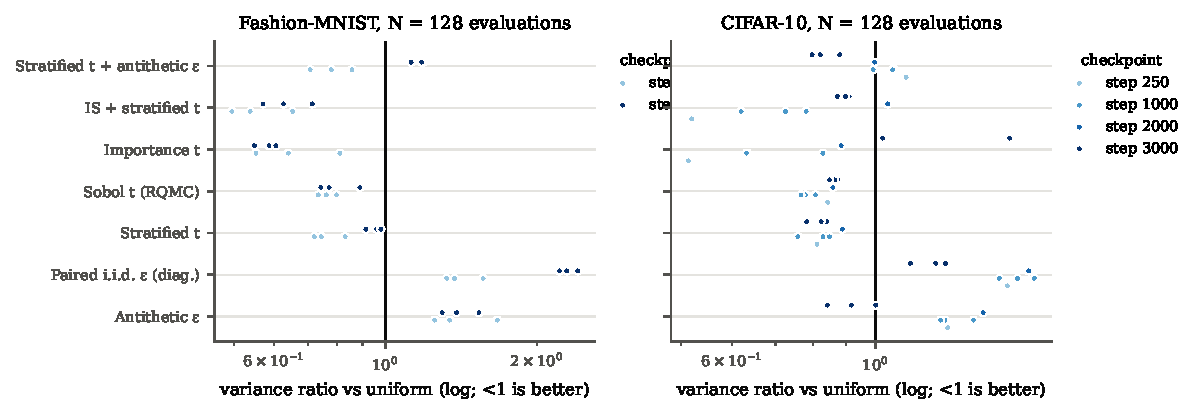
\includegraphics[width=\linewidth]{figures/var_ratio.pdf}
  \caption{\textbf{Gradient variance relative to uniform sampling at the same parameters and the same $N=128$.}
  Each dot is one (seed, checkpoint) probe with $R=48$ independent mini-batch gradients per estimator; colour
  shades mark the checkpoint. Values below 1 mean less variance. Stratified and Sobol timesteps are below 1
  everywhere. Antithetic noise is above 1 at most checkpoints, but always below its paired-i.i.d. control.
  Importance sampling moves from well below 1 to above 1 as training proceeds.}
  \label{fig:var}
\end{figure}

\paragraph{Gradient variance (Fig.~\ref{fig:var}, Table~\ref{tab:var}).}
\emph{Stratification works, but the gain is small.} On CIFAR-10, stratified timesteps give a variance ratio of
\StratVR\ at step 3000 (mean $\pm$ sd over 3 seeds) and \StratVRmin--\StratVRmax\ across all probes; the ratio is
below 1 in \StratVRbelow\ probes. Scrambled
Sobol timesteps behave the same (\SobolVR, \SobolVRbelow), as expected in one dimension (H1). The gain is
bounded by the between-timestep share of the variance, which is only \DecT\% (\S\ref{sec:where}).
\emph{Antithetic noise does not reduce variance at equal compute.} Its ratio is \AntiVR\ at step 3000 and
\AntiVRmin--\AntiVRmax\ over all probes (below 1 in \AntiVRbelow). The paired-i.i.d.\ control, which differs from
antithetic sampling only in the sign coupling, is far worse (\PairedVR), so the coupling works as intended.
What antithetic sampling cancels is roughly what it loses by sharing $(x_0,t)$ within a pair.
\emph{Importance sampling helps early and hurts late.} The loss-based proposal halves the variance at the first
probe (minimum ratio \ImpVRmin) but reaches \ImpVRmax\ by the end. Stratifying the IS uniforms stabilises it
(\ISSVR\ at step 3000; below 1 in \ISSVRbelow\ probes). On Fashion-MNIST, stratification, Sobol and
antithetic sampling behave the same way (\FStratVRmin--\FStratVRmax, \FSobolVRmin--\FSobolVRmax\ and
\FAntiVRmin--\FAntiVRmax). Importance sampling, however, reduces variance at every probe there
(\FImpVRmin--\FImpVRmax). Its late-training reversal is therefore specific to CIFAR-10 in our data, and the
800-step Fashion-MNIST runs may simply end before the proposal drifts. The unbiasedness check passes for every estimator
(\S\ref{sec:setup}).

\begin{table}[t]
  \centering\small
  \caption{\textbf{Gradient-variance ratio vs.\ uniform} ($\mathrm{tr}\,\mathrm{Cov}$, same $\theta$, $N=128$), mean $\pm$ sd over
  seeds. CIFAR-10 steps 250/2000 are seed 0 only, steps 1000/3000 have 3 seeds; Fashion-MNIST has 3 seeds.}
  \label{tab:var}
  \resizebox{\linewidth}{!}{\begin{tabular}{lrrrrrrrr}
\toprule
Estimator & fmnist @200 & fmnist @800 & cifar10 @250 & cifar10 @1000 & cifar10 @2000 & cifar10 @3000 & fmnist geo-mean [95\% CI] & cifar10 geo-mean [95\% CI] \\
\midrule
Antithetic $\epsilon$ & 1.42 $\pm$ 0.22 & 1.40 $\pm$ 0.12 & 1.29 & 1.32 $\pm$ 0.08 & 1.46 & 0.92 $\pm$ 0.08 & 1.41 [1.25, 1.58] & 1.16 [0.98, 1.38] \\
Paired i.i.d. $\epsilon$ (diag.) & 1.42 $\pm$ 0.13 & 2.31 $\pm$ 0.10 & 1.60 & 1.65 $\pm$ 0.10 & 1.72 & 1.22 $\pm$ 0.08 & 1.81 [1.35, 2.41] & 1.47 [1.28, 1.70] \\
Stratified t & 0.77 $\pm$ 0.06 & 0.95 $\pm$ 0.03 & 0.81 & 0.81 $\pm$ 0.05 & 0.89 & 0.82 $\pm$ 0.03 & 0.85 [0.74, 0.98] & 0.82 [0.79, 0.86] \\
Sobol t (RQMC) & 0.77 $\pm$ 0.03 & 0.80 $\pm$ 0.08 & 0.84 & 0.78 $\pm$ 0.02 & 0.86 & 0.86 $\pm$ 0.01 & 0.78 [0.73, 0.84] & 0.83 [0.80, 0.86] \\
Importance t & 0.67 $\pm$ 0.13 & 0.58 $\pm$ 0.03 & 0.51 & 0.70 $\pm$ 0.11 & 0.88 & 1.22 $\pm$ 0.34 & 0.62 [0.53, 0.72] & 0.84 [0.62, 1.14] \\
IS + stratified t & 0.56 $\pm$ 0.08 & 0.64 $\pm$ 0.07 & 0.52 & 0.71 $\pm$ 0.08 & 1.04 & 0.89 $\pm$ 0.02 & 0.60 [0.52, 0.69] & 0.78 [0.64, 0.94] \\
Stratified t + antithetic $\epsilon$ & 0.78 $\pm$ 0.07 & 1.16 $\pm$ 0.03 & 1.11 & 1.04 $\pm$ 0.04 & 1.00 & 0.83 $\pm$ 0.04 & 0.95 [0.75, 1.21] & 0.96 [0.86, 1.07] \\
\bottomrule
\end{tabular}
}
\end{table}

\begin{figure}[t]
  \centering
  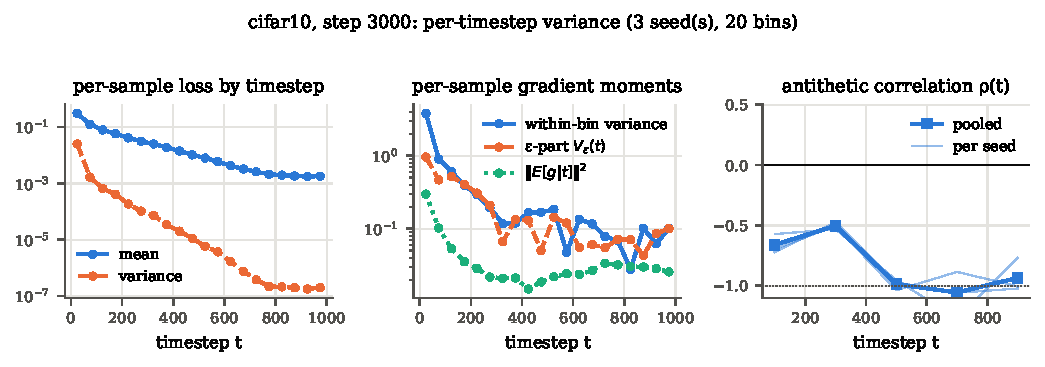
\includegraphics[width=\linewidth]{figures/per_t_cifar10.pdf}
  \caption{\textbf{Where the variance comes from (CIFAR-10, step 3000, 3 seeds).} Left: the per-sample loss and
  its variance fall by orders of magnitude from $t=0$ to $t=T$. Middle: the per-sample gradient moments vary far
  less. Right: the correlation between the gradients for $\epsilon$ and $-\epsilon$ (pooled over 4 bins and
  over seeds; thin lines are single seeds) is strongly negative at all $t$.}
  \label{fig:pert}
\end{figure}

\paragraph{Where the variance lives (Fig.~\ref{fig:pert}, Table~\ref{tab:decomp}).}
\label{sec:where}
On CIFAR-10 at step 3000, the per-sample gradient variance splits into \DecT\% between timesteps ($V_t$),
\DecX\% from the data given $t$ ($V_x$) and \DecE\% from the noise ($V_\epsilon$). This split explains the
results above. Stratifying $t$ can remove at most the 6\% between-timestep part plus some within-bin variation.
Antithetic noise attacks $V_\epsilon$ efficiently: $\rho=\Decrho$, close to the $-1$ of a locally affine network.
But by Eq.~\eqref{eq:anti} it helps only if $V_t+V_x<-\rho V_\epsilon$, and here
$V_t+V_x=\DecLHS$ while $-\rho V_\epsilon=\DecRHS$ (as fractions of the total). The condition fails, and it
fails more clearly on Fashion-MNIST, where the data term dominates ($V_x=\FDecX$\%, $\FDecLHS$ vs $\FDecRHS$).
The decomposition gets the ranking of the estimators right and predicts the absolute uniform variance to within
10\% on CIFAR-10. It overestimates the antithetic penalty at step 3000 (predicted \DecpAnti, measured \AntiVR).
For importance sampling, the loss-based proposal
$q\propto\sqrt{\mathbb E[\ell^2\mid t]}$ inherits the loss's $\approx$\LossRange$\times$ dynamic range across timesteps
(ratio of the largest to smallest bin), whereas $\sqrt{\mathbb E\|g\|^2\mid t}$ varies only $\approx$\GradRange$\times$. The
proposal therefore over-samples small $t$ and gives large weights to the rest. The gradient-optimal proposal
$q^\star$ would give a predicted ratio of \Decoracle\ on CIFAR-10 (\FDecoracle\ on Fashion-MNIST), the largest
reduction available from any timestep-only method here. This is a prediction, not a trained result.

\begin{table}[t]
  \centering\small
  \caption{\textbf{Law-of-total-variance decomposition and the variance ratios it predicts} (Eq.~\ref{eq:anti}),
  compared with the direct measurement at the same checkpoint. The last column is the absolute per-sample
  variance of the uniform estimator ($N\cdot\mathrm{tr}\,\mathrm{Cov}$), predicted and measured.}
  \label{tab:decomp}
  \resizebox{\linewidth}{!}{\begin{tabular}{lrrrrrr}
\toprule
 & stratified & antithetic & paired i.i.d. & strat+anti & oracle grad-IS & $N\,\mathrm{tr}\,\mathrm{Cov}$ (unif.) \\
\midrule
\multicolumn{7}{l}{\textit{Fashion-MNIST, step 800, 2 seed(s)}} \\
fractions $V_t / V_x / V_\epsilon$ & \multicolumn{6}{l}{5\% / 66\% / 30\%\quad pooled $\rho$ = -0.83 $\pm$ 0.14\quad $V_t+V_x$ = 0.70 vs $-\rho V_\epsilon$ = 0.25} \\
predicted ratio & 0.95 $\pm$ 0.00 & 1.46 $\pm$ 0.12 & 1.70 $\pm$ 0.04 & 1.36 $\pm$ 0.12 & 0.46 $\pm$ 0.05 & 2.170 $\pm$ 0.272 \\
measured ratio & 0.97 $\pm$ 0.01 & 1.41 $\pm$ 0.17 & 2.35 $\pm$ 0.08 & 1.16 $\pm$ 0.05 & -- & 1.642 $\pm$ 0.112 \\
\midrule
\multicolumn{7}{l}{\textit{CIFAR-10, step 3000, 3 seed(s)}} \\
fractions $V_t / V_x / V_\epsilon$ & \multicolumn{6}{l}{6\% / 44\% / 50\%\quad pooled $\rho$ = -0.71 $\pm$ 0.05\quad $V_t+V_x$ = 0.50 vs $-\rho V_\epsilon$ = 0.36} \\
predicted ratio & 0.94 $\pm$ 0.02 & 1.15 $\pm$ 0.05 & 1.50 $\pm$ 0.03 & 1.03 $\pm$ 0.05 & 0.62 $\pm$ 0.03 & 0.405 $\pm$ 0.011 \\
measured ratio & 0.82 $\pm$ 0.03 & 0.92 $\pm$ 0.08 & 1.22 $\pm$ 0.08 & 0.83 $\pm$ 0.04 & -- & 0.438 $\pm$ 0.012 \\
\bottomrule
\end{tabular}
}
\end{table}

\begin{table}[t]
  \centering\small
  \caption{\textbf{Training outcomes on CIFAR-10 at equal steps (3000) and equal evaluations per step.} Mean $\pm$ sd over
  seeds. $p$: two-sided Welch $t$-test against uniform (pre-registered). FID@1000/2000 are seed 0 only. The
  \ttt{strat\_anti} seed-2 run was trained without FID (PLAN A5), so its FID uses 2 seeds. ms/step excludes
  evaluation; T4 GPU, fp16.}
  \label{tab:main}
  \resizebox{\linewidth}{!}{\begin{tabular}{lrrrrrrrrr}
\toprule
Estimator & seeds & ms/step & overhead & held-out ($\times 10^{-3}$) & $p$ & FID@1000 & FID@2000 & FID@3000 & $p$ (FID) \\
\midrule
Uniform (baseline) & 3 & 90.8 & +0.0\% & 37.50 $\pm$ 0.18 & -- & 271.7 & 191.1 & 141.0 $\pm$ 5.7 & -- \\
Antithetic $\epsilon$ & 3 & 91.0 & +0.2\% & 37.75 $\pm$ 0.02 & 0.14 & 269.6 & 190.7 & 143.3 $\pm$ 3.0 & 0.58 \\
Stratified t & 3 & 90.4 & -0.5\% & 37.70 $\pm$ 0.22 & 0.29 & 270.2 & 190.5 & 140.0 $\pm$ 2.8 & 0.80 \\
Importance t & 3 & 92.2 & +1.5\% & 36.92 $\pm$ 0.32 & 0.07 & 269.1 & 184.8 & 135.3 $\pm$ 4.1 & 0.24 \\
Stratified t + antithetic $\epsilon$ & 3 & 89.4 & -1.6\% & 37.65 $\pm$ 0.19 & 0.37 & 271.7 & 189.3 & 141.2 $\pm$ 3.7 & 0.96 \\
\bottomrule
\end{tabular}
}
\end{table}

\begin{figure}[t]
  \centering
  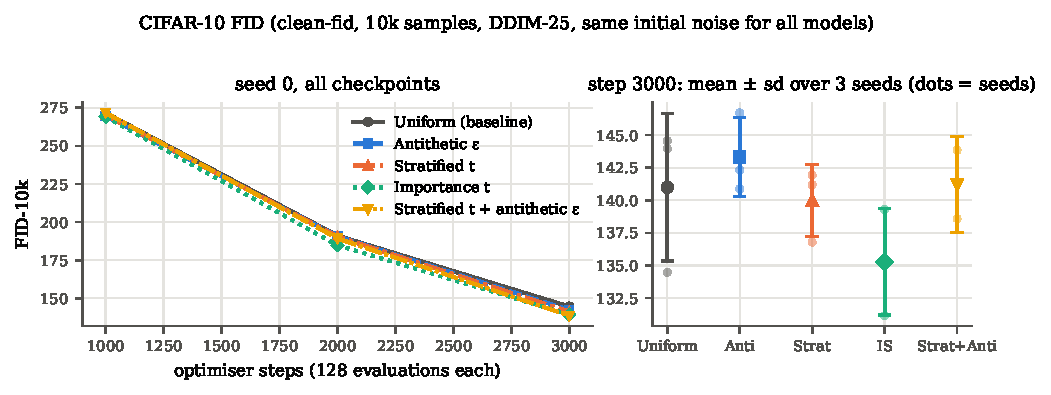
\includegraphics[width=\linewidth]{figures/fid_vs_steps_cifar10.pdf}
  \caption{\textbf{FID vs training steps (CIFAR-10).} Left: all checkpoints for seed 0. Right: step 3000, mean $\pm$ sd
  over seeds (dots are individual seeds). All estimators lie within one seed-to-seed standard deviation of uniform.}
  \label{fig:fid}
\end{figure}

\begin{figure}[t]
  \centering
  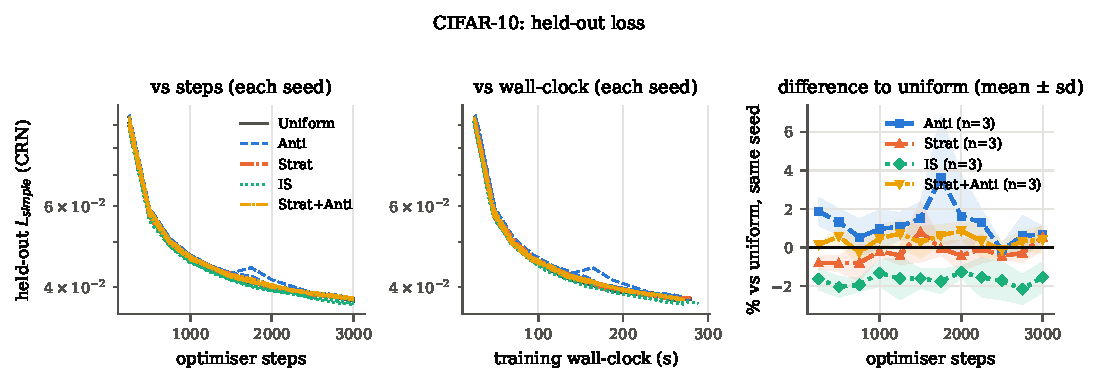
\includegraphics[width=\linewidth]{figures/loss_curves_cifar10.pdf}
  \caption{\textbf{Held-out loss (common random numbers) vs steps and vs wall-clock, CIFAR-10.} Right: relative difference
  to uniform for the same seed (same initialisation), mean $\pm$ sd. Importance sampling is consistently about
  1.5\% lower. The difference is not significant under the pre-registered test.}
  \label{fig:loss}
\end{figure}

\paragraph{Training outcomes (Table~\ref{tab:main}, Figs.~\ref{fig:fid}--\ref{fig:loss}).}
\emph{No estimator changes training outcomes significantly} (with 3 seeds, differences smaller than
$\approx$\MDEho\% in held-out loss or $\approx$\MDEfid\ FID are below the detection limit; \S\ref{sec:limitations}). At step 3000 the held-out loss
($\times10^{-3}$) is \UnifHO\ for uniform, \StratHO\ for stratified ($p=\StratpHO$), \AntiHO\ for antithetic
($p=\AntipHO$), \SAHO\ for stratified+antithetic ($p=\SApHO$) and \ImpHO\ for importance sampling
($p=\ImppHO$). FID-10k is \UnifFID\ (uniform), \StratFID, \AntiFID, \SAFID\ and \ImpFID\ respectively
(all $p\ge\ImppFID$). The 15--20\% variance reduction from stratification does not register in either metric.
Its effect on the held-out loss (\StratHOdiff\%) is far below the seed spread. Importance sampling is
best on both metrics despite \emph{higher} gradient variance late in training. In a secondary analysis that
pairs runs by seed (same initialisation and the same evaluation noise; not pre-registered), the differences
are \ImpHOpair\% in held-out loss ($p=\ImppHOpair$) and \ImpFIDpair FID ($p=\ImppFIDpair$). This is
suggestive but not significant. Gradient clipping was never active after warm-up in any arm (logged gradient
norms $\ll 1$), so clipping bias does not explain it. Two \emph{conjectures} we could not test within budget:
(a) the large early-training variance reduction (\ImpVRmin) gives IS a head start that persists; (b) because Adam
normalises each coordinate, re-allocating samples towards small $t$ changes the effective step size per
timestep, even though the gradient estimator is unbiased.
\emph{Overhead is negligible.} All estimators run at \UnifMS--\ImpMS\ ms/step (within $\pm$3\% of
uniform, inside timing noise), so loss vs wall-clock and loss vs steps are the same comparison.

\paragraph{Fashion-MNIST.} The CPU runs (\FSteps\ steps, 3 seeds) show the same pattern. Held-out loss
($\times10^{-3}$) is \FUnifHO\ (uniform), \FStratHO\ (stratified), \FAntiHO\ (antithetic), \FSAHO\ (strat+anti)
and \FImpHO\ (importance), with pre-registered $p$-values \FStratpHO, \FAntipHO, \FSApHO\ and \FImppHO. The
table is in Appendix~\ref{app:fmnist}.


\section{Limitations}
\label{sec:limitations}
\begin{itemize}\setlength\itemsep{2pt}
\item \textbf{Scale.} The models are small (1.5M / 0.6M parameters) and trained briefly (\Steps\ steps on CIFAR-10,
\FSteps\ on Fashion-MNIST) because of the 2-GPU-hour budget. FIDs around 140 mean the models are far from
converged. Gradient-noise effects may matter more, or less, late in training and at scale; we cannot tell
which. The variance \emph{measurements}, in contrast, are exact statements about these estimators at these
parameters.
\item \textbf{Power.} With three seeds per arm, a two-sided test at $\alpha=0.05$ has 80\% power only for effects of
about \MDEd\ within-arm standard deviations. Here that is $\approx$\MDEho\% in held-out loss or $\approx$\MDEfid\ FID points.
A non-significant result therefore rules out only large effects; it is not evidence of equivalence. The
importance-sampling difference (\ImpHOdiff\% held-out loss) is just below this threshold.
\item \textbf{FID protocol.} Because of the budget, FID was computed at three checkpoints for seed 0 and only at
the final checkpoint for seeds 1--2 (PLAN amendment A4). We used DDIM-25 rather than DDIM-50, 10k rather than
50k samples, and training-set statistics. All of these are fixed across arms, but they make the absolute values
incomparable to the literature.
\item \textbf{One optimiser, one weighting.} Everything uses Adam with $L_{\text{simple}}$. Adam's per-coordinate
normalisation may absorb part of the benefit of lower gradient variance \citep{jeha2024taylor}. Other loss
weightings (e.g.\ ELBO or Min-SNR \citep{hang2023minsnr}) change the per-timestep profile, and with it
$V_t$, and could favour stratification or importance sampling more.
\item \textbf{Importance proposal.} We trained only the Improved-DDPM loss-based proposal. The gradient-norm
oracle is evaluated analytically from the decomposition, not trained. Its predicted gain is a conjecture until
it is trained with an online estimate of $\mathbb E[\|g\|^2\mid t]$.
\item \textbf{Decomposition noise.} Per-bin estimates use 3 repetitions of single mini-batch differences, so
individual bins are noisy (single-bin $\rho$ can fall outside $[-1,1]$). We report ratio-of-sums pooled
estimates. The predicted uniform-estimator variance matches the direct measurement to within a few percent
on CIFAR-10 but less well on Fashion-MNIST (Table~\ref{tab:decomp}).
\item \textbf{Control variates} (item 5 of the original brief) were not implemented.
\end{itemize}


\section{Conclusion}
Classical variance reduction transfers to diffusion training in the sense that the estimators are unbiased,
cheap and act as theory predicts. In this regime they do not translate into better models at equal compute.
The law-of-total-variance decomposition explains why. The DDPM gradient's variance is dominated by data and
noise \emph{within} a timestep, not by the choice of timestep, which caps what stratification can achieve. Antithetic
noise cancels the noise term efficiently, but pays for it by halving the number of distinct images. The finance
lesson that transfers is diagnostic: measure the variance components first, then choose the estimator. The
most promising direction the measurements point to is a gradient-norm-based importance proposal, measured
post hoc at $\approx$\PHOracle$\times$ the baseline variance at fixed parameters, combined with stratification.
The only training-outcome signal, a 1.5--3\% held-out-loss gain from loss-based importance sampling, is
consistent across both datasets but not conclusive. That is a conjecture to test at larger
scale and with more seeds.


\bibliographystyle{abbrvnat}
\bibliography{references}

\appendix
\section{Compute budget and provenance}
\label{app:budget}
All GPU work ran as private Kaggle script kernels on T4$\times$2 machines, with two independent runs in
parallel, one per GPU. GPU usage was read from the Kaggle quota API before and after every session
(\texttt{results/budget.json}). Total: \GPUhours\ GPU-hours of the 2.0 available. The first smoke test spent its
entire 25-minute session downloading CIFAR-10 from the authors' server at $\sim$90\,kB/s (\GPUhoursLost\
GPU-hours, no training). We then switched to the Hugging Face mirror of the same images. Each kernel embeds
the exact source files and prints their SHA-256 hashes, which match the git commit named in every run's
\texttt{meta.json}. Results return through the kernel log as a checksummed archive
(\texttt{scripts/fetch\_kaggle\_results.py}). Every run is listed in \texttt{results/runs.csv} with its configuration,
seed, runtime, metrics and kernel URL. Every table, figure and in-text number is regenerated by
\texttt{scripts/make\_tables.py}, \texttt{make\_figures.py} and \texttt{make\_numbers.py}.

\section{Pre-registered plan and deviations}
\texttt{PLAN.md} was committed before any run. All deviations are listed there as amendments A1--A4, with
their reasons: model width 64$\to$32 and DDIM-50$\to$25 after measured timings, EMA warm-up, Fashion-MNIST
schedule, and a reduced FID schedule for seeds 1--2. No seed or run was excluded.

\end{document}
